Curvas de nível servem para representar dados tridimensionais em um plano. As três variáveis para esse tipo de gráfico são $x$ e $y$ independentes e $z = f(x,y)$.

Serão usados, como exemplo, dados semelhantes aos do experimento sobre potencial elétrico entre barras de cobre em uma solução condutiva. Nesse caso, as variáveis dependentes são as distâncias $x$ e $y$ no plano e a variável dependente é o potencial $V$ de cada ponto.

\begin{figure}[htbp]
    \centering
    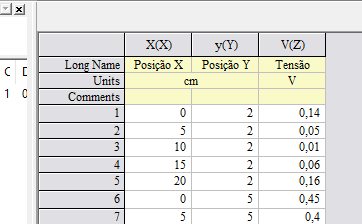
\includegraphics[width=0.4\textwidth]{contorno/1dados.png}

    \caption{Montagem dos dados de potencial na tabela do \software}
    \label{fig:contorno:dados}
\end{figure}


\subsection{Iniciando o Gráfico}

    \begin{figure}[htbp]
        \centering
        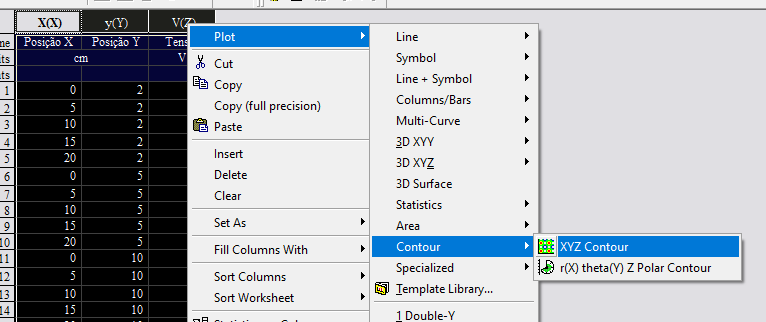
\includegraphics[width=0.8\textwidth]{contorno/2plot.png}

        \caption{Desenhando o gráfico de linhas de contorno}
        \label{fig:contorno:plot}
    \end{figure}

\subsection{Opções de Formatação}

    \begin{figure}[H]
        \centering
        \begin{subfigure}{0.7\textwidth}
            \centering
            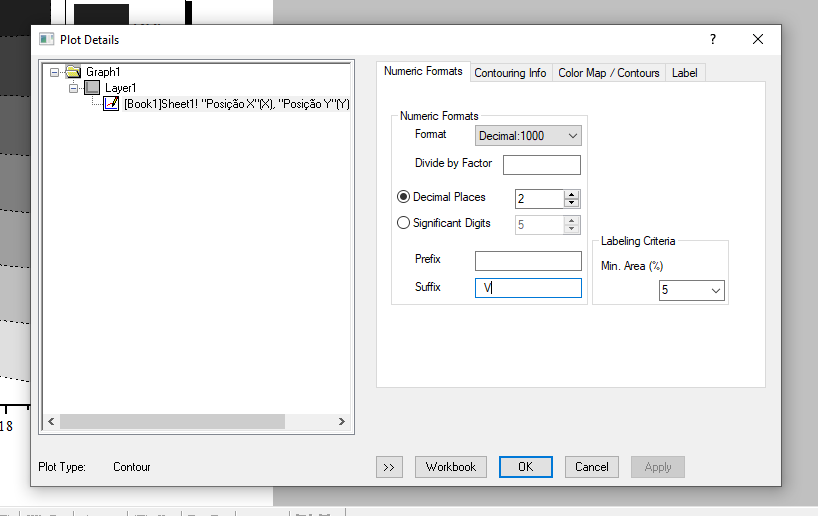
\includegraphics[width=\textwidth]{contorno/4sufixo.png}

            \caption{Adição de um sufixo nos dados em $z$}
            \label{fig:contorno:sufixo}
        \end{subfigure}
        ~
        \begin{subfigure}{0.7\textwidth}
            \centering
            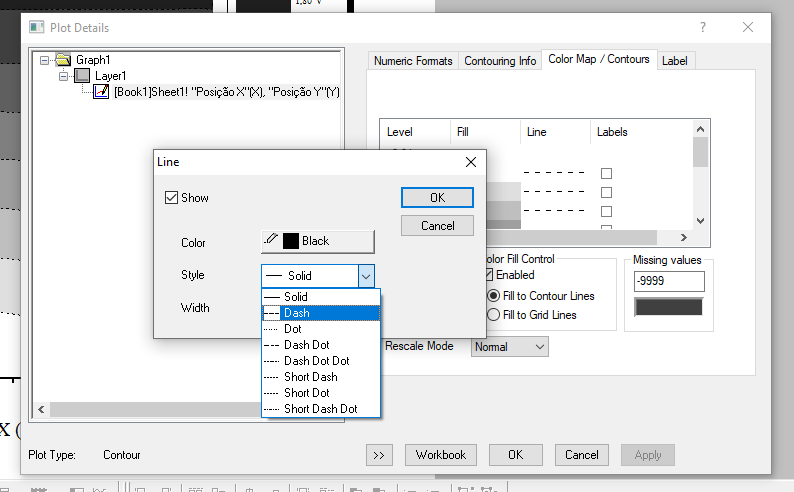
\includegraphics[width=\textwidth]{contorno/6linha.png}

            \caption{Mudança do estilo das linhas de separação dos níveis}
            \label{fig:contorno:linhas}
        \end{subfigure}
        \caption{Opções do gráfico de curvas de nível}
        \label{fig:contorno:opcoes}
    \end{figure}

    \begin{lembrete}
        É importante a adição de sufixos com a unidade do valor medido (figura \ref{fig:contorno:sufixo}).
    \end{lembrete}

    Para as paletas de cores existem muitas opções e vale mais a pena testar qual paleta funciona melhor com os seus dados. A caixa de opções é acessada como na figura \ref{fig:contorno:paleta}. A caixa da figura \ref{fig:contorno:escala} é acessada com um clique duplo na caixa com os níveis do eixo $z$.

    \begin{figure}[H]
        \centering
        \begin{subfigure}{0.45\textwidth}
            \centering
            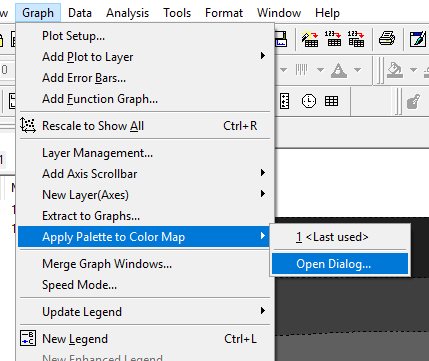
\includegraphics[width=\textwidth]{contorno/3paleta.png}

            \caption{Mudança da paleta de cores}
            \label{fig:contorno:paleta}
        \end{subfigure}
        ~
        \begin{subfigure}{0.45\textwidth}
            \centering
            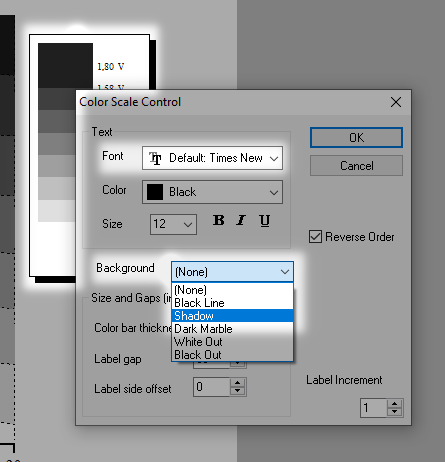
\includegraphics[width=\textwidth]{contorno/5bg.png}

            \caption{Opções da escala de níveis}
            \label{fig:contorno:escala}
        \end{subfigure}
        \caption{Mais opções de formatação}
        \label{fig:contorno:extra}
    \end{figure}

\subsection{Resultado}

    \begin{figure}[htbp]
        \centering
        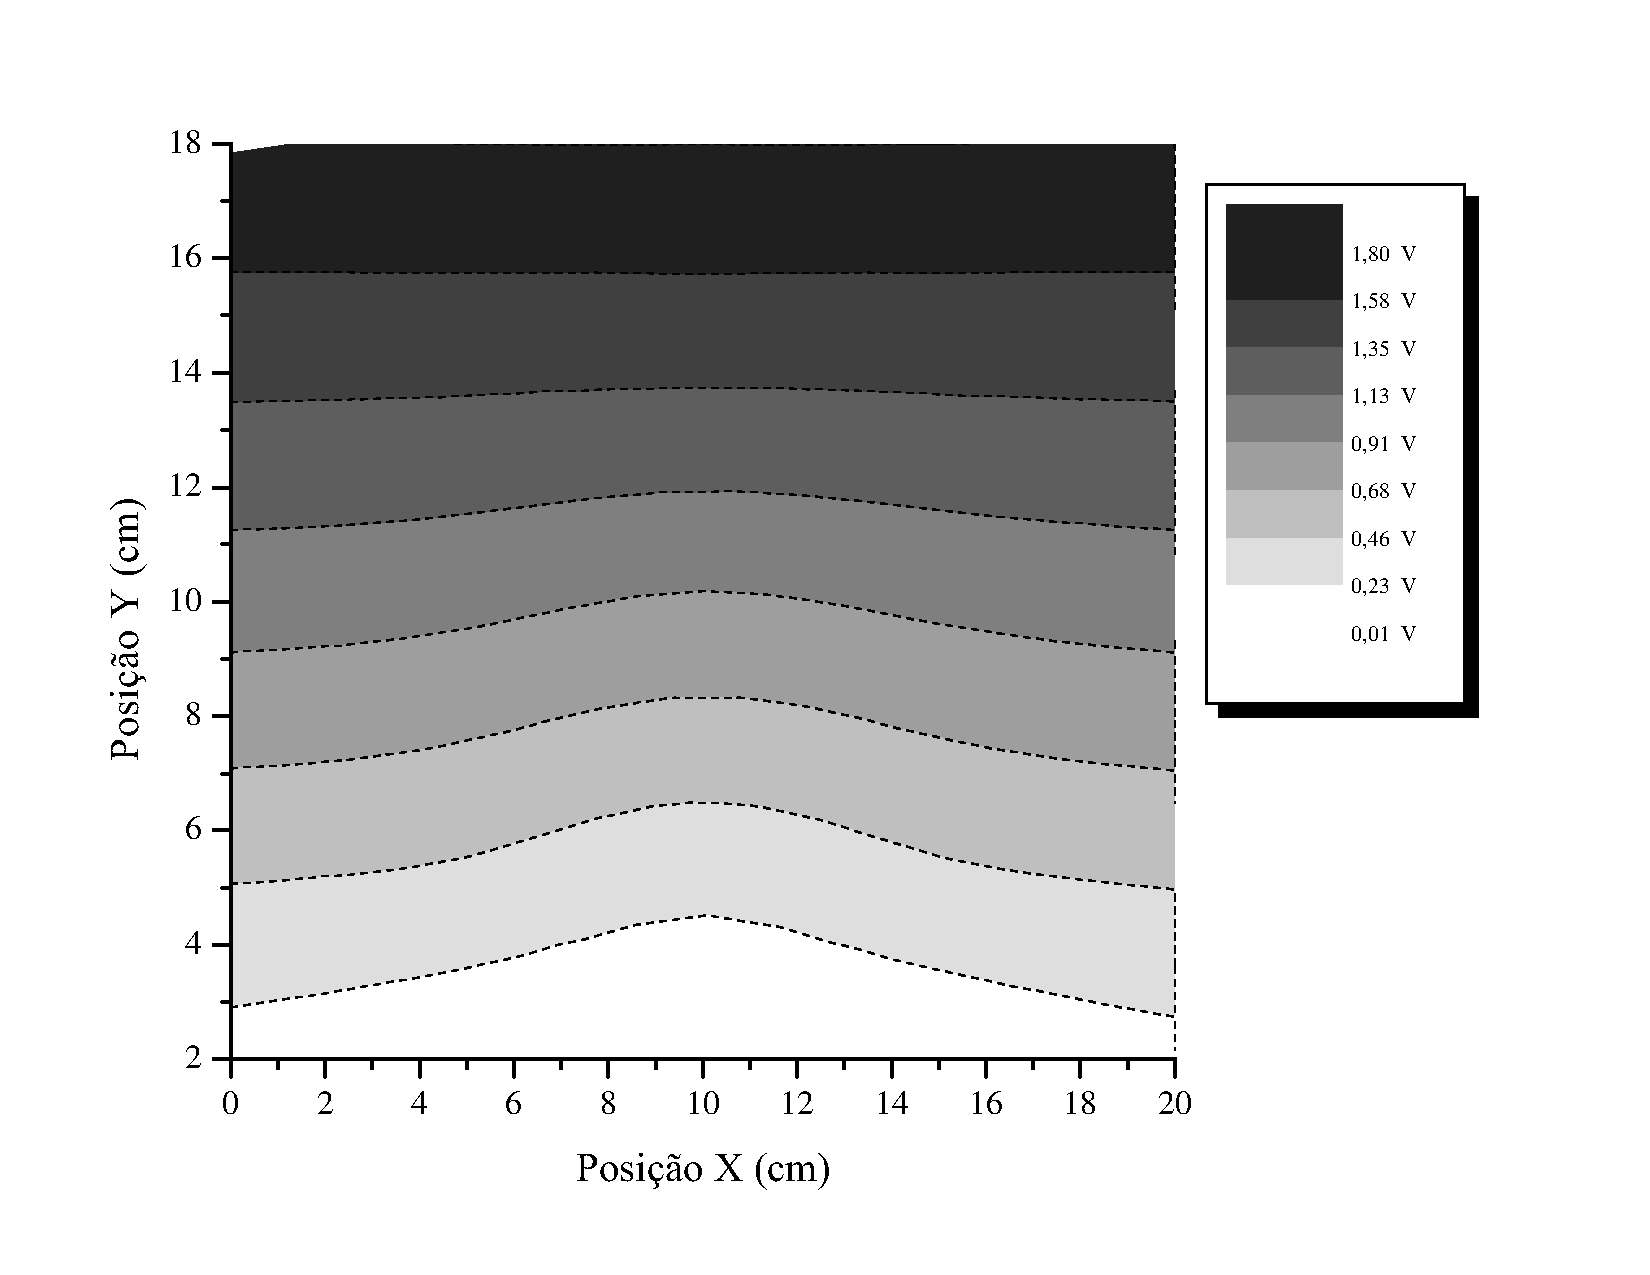
\includegraphics[width=0.9\textwidth]{contorno/resultado.pdf}

        \caption{Deformação das equipotenciais gerada pela adição de uma ponta}
        \label{fig:contorno:final}
    \end{figure}

